\documentclass[10pt,conference,compsoc]{IEEEtran}

\usepackage{amsmath}
\usepackage{booktabs}
\usepackage{graphicx}
\usepackage{microtype}
\usepackage{newtxtext,newtxmath}
\usepackage{url}

\graphicspath{{../../figures/}}

\title{Benchmarking Rule-Based, Learned, and Zero-Shot GPT-4o Grasp Prediction Under a Unified Evaluation Protocol}

\author{\IEEEauthorblockN{Anish Talla}
\IEEEauthorblockA{\textit{High School Student}\\
United States}}

\begin{document}
\maketitle

\begin{abstract}
I compared three ways to predict a robotic grasp from an RGB image: a
detector-assisted heuristic, a neural network trained on grasp labels, and
GPT-4o used zero-shot with one frozen prompt. All three systems saw the same
object-wise test split of the Cornell Grasping Dataset, returned the same
rectangle, and were scored by the same code. Supervision and tuning effort
were not equalized, and the paper says where that matters. A fine-tuned
ResNet18 passed on 79.7\% of test images, and a second training round with a
stable recipe and three seeds per architecture put the learned system at
84.0\%. The heuristic passed on 40.7\% before a post-hoc correction and
57.7\% after it. GPT-4o passed on 12.4\% of calls across five independent
runs per image. Object-clustered resampling left the order unchanged. The
errors differed. The heuristic, limited to two orientations, struggled with
angle. The ResNet18 usually missed on placement. GPT-4o failed both
criteria on 59.3\% of calls, and its predicted center lay outside the convex
hull of all labeled grasp corners on 53.4\% of parsed calls, against 7.0\%
and 6.5\% for the other systems. My first explanation was that the model
could see a grasp but not express it as coordinates. A fourth run tested
that directly by drawing label-free candidate grasps on the image and asking
the same model to choose one by number. On three candidate menus its
accuracy stayed at the random floor, and it kept preferring a grasp closing
along the object's long axis. The failure is in the grasp choice, not in
emitting coordinates.
\end{abstract}

\begin{IEEEkeywords}
robotic grasping, computer vision, deep learning, vision-language models,
multimedia data mining, spatial grounding
\end{IEEEkeywords}

\section{Introduction}

A robot has to make a geometric decision before it can close its gripper:
where the fingers should land, how the gripper should rotate, and how far the
jaws should open. A practitioner starting a grasping project has three cheap
options. Write the decision as rules on top of an off-the-shelf detector.
Train a small network on a few hundred labeled images. Or ask a
general-purpose VLM for the answer with no grasp training at all. Published
numbers for these options are not comparable, because each paper changes the
input modality, the output type, or the scoring rule along with the method.

I built one system of each kind and held three things fixed: every system
saw the same 123 held-out RGB images, returned one grasp rectangle, and was
scored against the same Cornell labels by one implementation of the standard
rectangle test \cite{jiang2011,lenz2015}. That is what ``unified'' means in
this paper. It does not mean equal supervision or equal tuning: the network
is trained on Cornell labels, the heuristic is handed a detector and a
segmentation, and the VLM gets one prompt. The comparison is between
complete pipelines, and the budget differences are stated where they matter.

Two factors are the focus. The first is orientation. The heuristic can emit
only $0^\circ$ or $90^\circ$, and the learned system regresses a continuous
angle, so the gap between them isolates what a continuous orientation head
buys. The second is the VLM's output interface. When a VLM scores poorly on
raw coordinates, the failure could sit in choosing a grasp or in expressing
that choice as pixels. A fourth run separates the two by removing the
coordinate output entirely. Everything else that differs between the
systems is treated as context, not as a controlled variable.

The contribution is threefold: a controlled comparison on an object-wise
split with object-clustered inference; a shared failure taxonomy with a
center-hull check that locates where each system fails; and a hypothesis
test whose result overturned the explanation I first proposed for the VLM.
Dense grasp detectors already report higher Cornell scores \cite{kumra2020}.
The aim here is different: compare three practical starting points without
changing the test when the method changes.

\section{Related Work}

Jiang \emph{et al.} introduced the Cornell dataset and its rectangle
representation of a grasp \cite{jiang2011}. Under the usual test, a
prediction passes when it is within $30^\circ$ of a labeled grasp and its
intersection over union (IoU) exceeds 25\% \cite{lenz2015}; the two-stage
deep network of Lenz \emph{et al.} reached 75.6\% object-wise with RGB-D
input. Redmon and Angelova regressed one rectangle with a network and
reported 84.9\% object-wise, again with depth \cite{redmon2015}. System B
follows their single-rectangle formulation but uses RGB only, so that all
three systems share one input. GR-ConvNet and other pixel-wise models
report higher scores, but they make a dense prediction instead of
regressing one rectangle for the whole image \cite{kumra2020}; I do not
compare against them.

VLM-based grasping systems usually do not ask the language model for the
final pixel coordinates. Set-of-Mark prompting has the model choose among
regions already marked on an image \cite{yang2024}. VLAD-Grasp has a VLM
draw the grasp, then recovers a pose with depth prediction, segmentation,
and point-cloud alignment \cite{kulshrestha2025}. System C removes all of
that scaffolding and asks GPT-4o for the coordinates directly; System D adds
back the simplest possible scaffold, a numbered menu of candidates, without
any labels. Their scores describe those two output methods, not a limit on
VLM-based grasping.

\section{Experimental Design}

\subsection{Dataset, Split, and Metric}

Cornell contains 885 RGB-D images of household objects, with several positive
grasp rectangles on most images. I used only RGB.

Cornell does not include object IDs, so I reconstructed them from the frame
sequence. The procedure segmented the object from the photography platform
and compared consecutive masks with color and area descriptors that tolerate
rotation. I set the thresholds asymmetrically because the two possible
mistakes have different costs. If two objects are merged, the combined group
still stays in one split. If one object is split in two, its images can leak
into both training and test. Of 884 consecutive-frame boundaries, 478 were
accepted automatically as the same object and 155 as different objects. The
remaining 251 (28.4\%) fell in the ambiguous band or had a failed
segmentation, and were routed to manual review.

An AI assistant made a first pass over those 251, logging a decision and a
confidence for each. In a blind audit of 30 of them, its calls agreed with
mine on 86.7\% of confident cases and 40.0\% of uncertain ones, so I then
decided every uncertain call, every ``different object'' call, and every
call whose reasoning relied on a failed segmentation myself. Six boundaries
stayed ambiguous after that review. Four with a directional lean were
resolved toward ``same'', the low-risk direction. Two had no lean at all;
rather than guess, I excluded one image on the smaller side of each
boundary, leaving 883 images. Neither was an annotation error. Table
\ref{tab:split} shows the final seed-42 split. A second check confirmed
that no object appears in more than one partition.

\begin{table}[t]
\caption{Object-wise Cornell split.}
\label{tab:split}
\centering
\begin{tabular}{lrr}
\toprule
Partition & Objects & Images \\
\midrule
Train & 164 & 620 \\
Validation & 35 & 140 \\
Test & 35 & 123 \\
\midrule
Total & 234 & 883 \\
\bottomrule
\end{tabular}
\end{table}

I scored each prediction against every positive rectangle on its image. A
match to any one of them counts as correct. Before using the evaluator at
scale, I checked hand-computed cases, rectangle round trips, and an independent
rasterized IoU calculation. All predictions were converted back to the native
$640\times480$ coordinate frame for the final comparison.

\subsection{System A: Detector-Assisted Heuristic}

System A starts with a COCO-pretrained Faster R-CNN using a
ResNet50-FPN-v2 backbone \cite{ren2015}. A fixed lookup table maps the detected
category to a center, upper, or end grasp. I calibrated the global opening and
jaw-size constants on training labels only. The COCO vocabulary misses most
Cornell objects, so a platform-segmentation fallback supplies a box when the
detector cannot. The rule closes the gripper across the box's narrow
dimension. It can output only $0^\circ$ or $90^\circ$. That design limit
has a measurable ceiling: 118 of the 123 test images (95.9\%) have at least
one labeled grasp within the metric's $30^\circ$ tolerance of one of those
two angles, and 103 (83.7\%) have one within $15^\circ$. Only five test
images are unreachable at any placement, so the constraint caps System A
near 96\%, not near its score.

The first test run scored 40.7\%. Its rendered predictions exposed a defect:
some accepted detections covered background clutter instead of the object on
the platform. I added a guard requiring the detection to contain the
segmented object's centroid and recalibrated the global constants on training
data. The score rose to 57.7\%. Test output prompted that change, so 57.7\%
is post-hoc. All statistical comparisons below use the clean 40.7\% unless
labeled otherwise.

\subsection{System B: Learned Predictor}

System B replaces ResNet18's ImageNet classifier \cite{he2016} with separate
heads for center, orientation, and size. The orientation head predicts
$(\cos 2\theta,\sin 2\theta)$. Doubling the angle handles the fact that a
parallel-jaw grasp is unchanged by a $180^\circ$ rotation. For images with
several labels, I compute the loss against every rectangle and backpropagate
only the best match. Averaging all valid labels could put the target between
two good grasps, where neither one actually exists.

I trained a custom CNN, ResNet18, and ResNet34 on the 620 training images.
Affine augmentation moved the rectangle corners with the pixels. Architecture,
checkpoint, size-loss weight, and the custom CNN's learning rate were chosen
on validation data. ResNet18 had the best validation accuracy at 83.6\%, so I
froze that model before opening the test results.

That first round trained each architecture once, at one seed, with a
constant learning rate, and kept the best of roughly a hundred noisy
validation epochs. A second round kept the model, loss, data, and split and
changed only the recipe: cosine learning-rate decay over a fixed 100 epochs,
an exponential moving average of the weights, three seeds per architecture,
and no checkpoint selection. Test-time augmentation over eight dihedral
views, combined by taking the medoid rectangle, was adopted only because it
raised mean validation accuracy. Four selection rules were written down
before the test split was opened a second time, and every configuration
that touched test is reported. System B therefore received far more
development effort than Systems C and D, which each ran one frozen prompt.

\subsection{System C: Zero-Shot VLM}

System C sends the native RGB image to GPT-4o through OpenRouter
\cite{openai2024}. It uses no grasp-specific training. The prompt asks for two
fingertip coordinates and a jaw width in JSON, which together define the
rectangle. I developed the prompt on 30 training images and froze it before
test.

Each test image was sent in five independent, single-turn calls at the
provider's default temperature. I retried transport failures, but not replies
that arrived and failed to parse. Retrying those would quietly turn a
single-call baseline into a best-of-several system. Of 615 calls, 614 parsed.
The primary score pools the five exchangeable runs to estimate one-call
accuracy. Best-of-five is only a ceiling: it requires five calls and an oracle
that knows when one of them is right.

\subsection{System D: Marked-Candidate Selection}

If GPT-4o can see where to grasp but cannot express it as coordinates,
removing the coordinate output should recover its choice. System D shows the
same model the same test images with candidate grasps drawn on a zoomed crop
and asks for the number of the one it would use. Candidates come only from
the platform-segmentation mask: principal-component analysis gives the
centroid, long axis, and extent, and candidates are positions along the long
axis crossed with four jaw-travel directions $45^\circ$ apart, so every grasp
angle is within the metric's tolerance of some candidate. Opening and jaw
width use System A's train-calibrated constants. Numbering is re-shuffled on
every call. Because the menu is fixed before the model sees it, each run
carries its own floor (expected accuracy of a uniformly random choice) and
ceiling (whether any candidate passes).

Three menus were run, each on the full test split with five repeats: twelve
marks at three positions; four marks at the centroid drawn at real size; and
the same four marks drawn at one uniform length, with the prompt stating
that length is not to scale. The last two menus exist because on thin
objects the correct marks are the smallest on the image, so a preference
for large marks would mimic a preference for the long-axis grasp. The
prompt was developed on 30 training images for parse rate and glyph reading
only.

\subsection{Statistical and Failure Analysis}

The 123 test images are repeated views of 35 unseen objects, not 123
independent samples. I formed the 95\% confidence intervals from 20,000
object-clustered bootstrap resamples. Every view of an object, along with all
five VLM calls, moves together. Paired differences use the same resamples and
20,000 object-level label-swap permutations.

The failure analysis gives each attempt one label: correct, angle only,
overlap only, both criteria, or no prediction. I also checked whether the
predicted center falls inside the convex hull of all labeled grasp corners on
the image. This is a loose spatial check, not a claim that the grasp would
work on hardware. A center outside that hull falls beyond the area spanned by
the annotated grasp corners.

\section{Results}

\subsection{Overall Accuracy}

ResNet18 passed 98 of 123 images (79.7\%). The heuristic passed 50 before
its correction (40.7\%) and 71 after it (57.7\%). GPT-4o passed 76 of 615
calls (12.4\%); its five runs ranged from 9.8\% to 14.6\%. At least one
GPT-4o call passed on 43 of the 123 images, a best-of-five ceiling of
35.0\%. Table~\ref{tab:accuracy} gives the object-clustered intervals.

\begin{table}[t]
\caption{Accuracy with object-clustered 95\% confidence intervals. The
corrected System A row is post-hoc and is not used in the paired tests.}
\label{tab:accuracy}
\centering
\begin{tabular}{lrr}
\toprule
System & Accuracy & 95\% CI \\
\midrule
A: heuristic, pre-correction & 40.7\% & [28.0, 53.2] \\
A: heuristic, corrected (post-hoc) & 57.7\% & [46.2, 68.2] \\
B: ResNet18, round 1 & 79.7\% & [70.8, 87.1] \\
B: ResNet34, round 2, 3 seeds & \textbf{84.0\%} & [73.9, 92.1] \\
C: GPT-4o, one call & 12.4\% & [8.0, 17.4] \\
C: best of five & 35.0\% & [24.6, 45.5] \\
\bottomrule
\end{tabular}
\end{table}

Against the clean heuristic, ResNet18 led by 39.0 points, bootstrap
interval [25.2, 52.9], permutation $p<0.0001$. The clean
heuristic led GPT-4o's expected one-call score by 28.3 points
[16.9, 40.0], $p=0.0001$, and its best-of-five ceiling by 5.7
points [-6.1, 18.0], $p=0.45$; the last gap is the only one
whose interval includes zero. Using the post-hoc 57.7\% instead, the B--A
gap was 22.0 points [9.7, 35.1], $p=0.0031$, and A led best-of-five C by
22.8 points [9.2, 35.6], $p=0.0060$. Giving each object equal weight
produced 38.5\%, 75.4\%, and 10.5\% for clean A, B, and one-call C,
which changed the size of the gaps but not their order.

The second training round chose ResNet34 on mean final-weight validation
accuracy (81.4\% against 81.2\% for ResNet18). Its three seeds scored 84.6,
83.7, and 83.7\% on test, a mean of 84.0\% with interval [73.9, 92.1];
ResNet18 under the same recipe averaged 82.6\%. Re-running the first-round
recipe at two new seeds gave 82.9\% and 80.5\%, so 79.7\% was a low-side
single draw and the first round's nine-point gap between ResNet18 and
ResNet34 was run-to-run noise. Round 2's 4.3-point lead over round 1 does
not exclude zero. For a single-rectangle regressor without depth, these
scores sit between the 75.6\% of Lenz \emph{et al.} and the 84.9\% of
Redmon and Angelova, both obtained with depth input
\cite{lenz2015,redmon2015}.

\subsection{Failure Patterns}

The error counts in Table~\ref{tab:taxonomy} separate the systems more clearly
than accuracy alone. The correction moved System A mostly out of the
``both'' row: 20 of its clean run's 34 both-criteria failures came from
detector boxes the guard later rejected as off the object, and 14 of those
images passed once the segmentation fallback took over. Its angle-only
count barely changed, 15 before and 13 after, which fits a system limited
to two orientations. B had four angle-only failures. Fifteen of its 25 misses
failed only on overlap, so placement was the larger remaining problem. C
failed both tests on 365 of 615 calls (59.3\%).

\begin{table}[t]
\caption{Shared failure taxonomy. Percentages use all attempts. System A
is shown before (clean) and after (post-hoc) its correction.}
\label{tab:taxonomy}
\centering
\footnotesize
\setlength{\tabcolsep}{4pt}
\begin{tabular}{lrrrr}
\toprule
Outcome & A clean & A post-hoc & B & C \\
& ($n=123$) & ($n=123$) & ($n=123$) & ($n=615$) \\
\midrule
Correct & 50 (40.7) & 71 (57.7) & 98 (79.7) & 76 (12.4) \\
Angle only & 15 (12.2) & 13 (10.6) & 4 (3.3) & 85 (13.8) \\
Overlap only & 16 (13.0) & 18 (14.6) & 15 (12.2) & 88 (14.3) \\
Both & 34 (27.6) & 13 (10.6) & 6 (4.9) & 365 (59.3) \\
No prediction & 8 (6.5) & 8 (6.5) & 0 (0.0) & 1 (0.2) \\
\bottomrule
\end{tabular}
\end{table}

The center-hull check shows where C's failures begin. A landed outside the
labeled grasp hull on 8 of 115 predictions (7.0\%), and B did so on 8 of 123
(6.5\%). C did so on 328 of 614 parsed calls (53.4\%). Figure
\ref{fig:comparison} shows the shared coordinate frame on one image. This is
not an even contest by itself: A starts from a detected or segmented object,
and B was trained on Cornell. C can place its coordinates anywhere. I use
this check to locate a possible stage of failure. The three rates do not
estimate the same underlying capability.

\begin{figure}[t]
\centering
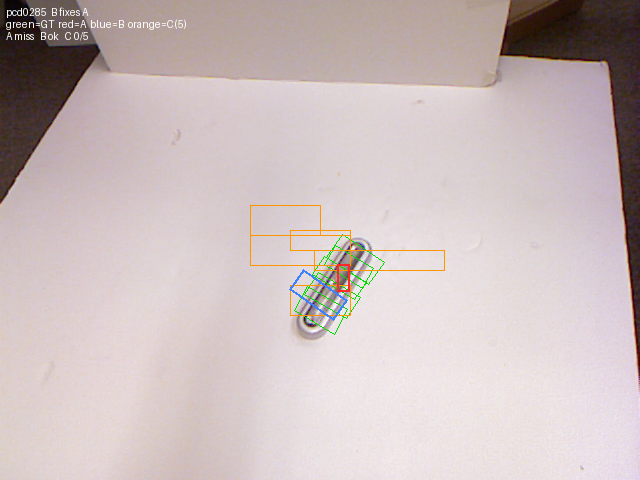
\includegraphics[width=\columnwidth]{compare_0285.png}
\caption{One test image under the shared coordinate system. Labeled grasps
are green, System A red, System B blue, and System C's five repeats orange.}
\label{fig:comparison}
\end{figure}

The five GPT-4o calls also disagreed with one another. Mean pairwise rectangle
agreement was 22.0\%, and mean pairwise IoU was 0.13. All five calls failed on
80 of 123 images. All five passed on one image. The remaining 42 images were
unstable: identical pixels sometimes produced a passing grasp and sometimes
did not.

\subsection{System D}

Table~\ref{tab:menus} gives the three menus. On none of them does the
model's one-call accuracy differ from a random choice among the same
candidates (paired object-clustered differences $-1.4$ [$-6.6$, $+4.0$],
$+1.9$ [$-2.2$, $+6.3$], and $-2.3$ [$-6.3$, $+1.7$]), while the ceilings
are 79.7\% and 65.9\%. Its choices are not random, though. On the full
menu it chose the candidate whose jaws travel along the object's long axis
near one end in 61\% of calls, a grasp type that passes 17\% of the time,
with reasoning such as ``grips the narrow top edge near the center of
mass''. With four marks at the centroid drawn at one uniform size, it still
chose the long-axis direction in 45\% of calls against a 25\% chance rate,
and the short-axis candidate, which passes on 55\% of images, in 17\%.
Stated confidence was ``high'' on 556 of 560 full-menu calls, 21\% of them
correct. Every reply parsed. The candidate at the centroid closing across
the short axis, with no model at all, scored 55.3\% [41.8, 68.0], level
with corrected System A.

\begin{table}[t]
\caption{System D on three candidate menus, same model and test images,
five repeats each. ``Long axis'' is the share of calls choosing the
orientation whose jaws travel along the object's long axis; chance is 25\%
on the four-mark menus.}
\label{tab:menus}
\centering
\footnotesize
\begin{tabular}{lrrrrr}
\toprule
Menu & Marks & Acc. & Floor & Ceil. & Long axis \\
\midrule
Full, 3 positions & 12 & 18.7 & 20.1 & 79.7 & 70\% \\
Centroid, real & 4 & 26.5 & 24.6 & 65.9 & 41\% \\
Centroid, uniform & 4 & 22.3 & 24.6 & 65.9 & 45\% \\
\bottomrule
\end{tabular}
\end{table}

\section{Discussion and Limitations}

On this setup, asking GPT-4o for raw coordinates worked poorly. This result
does not extend to VLM grasping methods in general. Set-of-Mark and VLAD-Grasp
use a VLM without making it emit the final coordinates, and both add machinery
that System C does not have \cite{yang2024,kulshrestha2025}.

On a sample of C's failures, I read rationales that named a plausible part of
the object while the coordinates landed elsewhere. Together with the 53.4\%
center-hull rate, that suggested a coordinate-binding explanation: the model
recognizes a useful region in words and loses it while mapping the answer
into pixels. Other explanations fit the same evidence, for instance that the
model does not understand the image's coordinate frame or scale. System D
was designed so that all of these would predict the same thing: with the
coordinate output removed and a menu whose ceiling is 79.7\%, the choice
should recover. It did not. Accuracy stayed at the menu's random floor, and
the preference for closing along the long axis survived menus with no
end-straddling candidates and with every mark the same size. From a
top-down photograph, two fingertip pads straddling the end of an elongated
object do look like they pinch a narrow part; in three dimensions the
second finger lands on top of the object. The failure is better described
as grasp reasoning from a single 2-D view than as text failing to bind to
coordinates.

The orientation result is more ordinary but useful. The two-angle
constraint itself removes only five test images from System A's reach,
because most Cornell images carry several labels and one of them is
usually near an axis. Its 13 angle-only failures are therefore mostly
cases of closing across the wrong one of the two axes, not of a diagonal
object that no axis-aligned grasp could fit. A continuous orientation
head fixes both: System B had four angle-only failures and a mean angle
error of $3.9^\circ$. System D's label-free candidate at the centroid,
closing across the segmented short axis, gets the same benefit without a
detector and matches corrected A.

In practice, these results argue for a specific order of operations. A
segmentation-based short-axis rule costs nothing to build and is the right
first baseline. When a few hundred labeled images exist, a fine-tuned
ResNet is worth the training and outperforms the rule by 20 to 40 points on
this benchmark. A raw-coordinate query to GPT-4o should not serve as a
grasp planner, and a numbered menu of candidates does not fix it on its own
with this model, so a VLM in the loop needs geometry supplied by other
means, as in the cited pipelines.

The experiment has several limits. It uses one object-wise split of a small
benchmark, RGB without depth, and no robot trials, and the 35-object test
set gives wide intervals. Cornell's annotations are not exhaustive, so a
rectangle that fails the metric might still work on a real object. System
B received more development effort than any other system: three
architectures, validation-based tuning, and a second training round,
compared with one frozen prompt for C and D. The test split was opened
twice for System B, once per round, under rules fixed beforehand, but two
openings are still two. System C tested one model and one prompt; System D
used one glyph style and one candidate generator. An early formatting check
on about 550 grasp rectangles probably included a few images that later
entered test, although no parameter or rule came from that check. Test
inspection prompted System A's correction, which is why its clean 40.7\%
anchors every paired test above. Confirmation requires a fresh split,
object-wise cross-validation, or a second dataset.

\section{Conclusion}

ResNet18 scored highest at 79.7\%, and 84.0\% averaged over three seeds
under a stable recipe. The heuristic reached 40.7\% clean and 57.7\% after
a post-hoc correction, and GPT-4o reached 12.4\% per call. On the two focal
factors: a continuous orientation head removed most of the heuristic's
angle-only failures, and taking the coordinate output away from GPT-4o did
not recover its grasp choice. The same model, given marked candidates,
chose no better than chance on three menus and kept preferring an end pinch
along the object's long axis even when every mark was drawn the same size.
The problem is the grasp choice, not its expression. What remains untested
is whether depth input, or a model with a stronger three-dimensional prior,
changes that choice.

\section*{Acknowledgment}

I designed the study, chose the three systems and the evaluation protocol,
built the object-wise split and audited its ambiguous boundaries, ran and
checked every experiment, verified all numerical claims and citations, and
wrote and approved the final text. AI coding assistants were used as tools
under my direction: OpenAI Codex edited and shortened the manuscript from my
draft and verified results, and Anthropic Claude Code helped implement
scripts, made a logged first pass on ambiguous object boundaries that I then
reviewed in full, and implemented the second training round and the System
D harness to my specification. GPT-4o is not an assistant here; it is the
model evaluated as Systems C and D.

\begin{thebibliography}{00}

\bibitem{jiang2011}
Y. Jiang, S. Moseson, and A. Saxena, ``Efficient grasping from RGBD images:
Learning using a new rectangle representation,'' in \emph{Proc. IEEE Int.
Conf. Robot. Autom. (ICRA)}, 2011, pp. 3304--3311.

\bibitem{lenz2015}
I. Lenz, H. Lee, and A. Saxena, ``Deep learning for detecting robotic
grasps,'' \emph{Int. J. Robot. Res.}, vol. 34, nos. 4--5, pp. 705--724, 2015.

\bibitem{redmon2015}
J. Redmon and A. Angelova, ``Real-time grasp detection using convolutional
neural networks,'' in \emph{Proc. IEEE Int. Conf. Robot. Autom. (ICRA)},
2015, pp. 1316--1322.

\bibitem{kumra2020}
S. Kumra, S. Joshi, and F. Sahin, ``Antipodal robotic grasping using
generative residual convolutional neural network,'' in \emph{Proc. IEEE/RSJ
Int. Conf. Intell. Robots Syst. (IROS)}, 2020, pp. 9626--9633.

\bibitem{yang2024}
J. Yang \emph{et al.}, ``Set-of-Mark prompting unleashes extraordinary
visual grounding in GPT-4V,'' \emph{arXiv:2310.11441}, 2023.

\bibitem{kulshrestha2025}
M. Kulshrestha \emph{et al.}, ``VLAD-Grasp: Zero-shot grasp detection via
vision-language models,'' \emph{arXiv:2511.05791}, 2025.

\bibitem{ren2015}
S. Ren, K. He, R. Girshick, and J. Sun, ``Faster R-CNN: Towards real-time
object detection with region proposal networks,'' in \emph{Adv. Neural Inf.
Process. Syst.}, vol. 28, 2015.

\bibitem{he2016}
K. He, X. Zhang, S. Ren, and J. Sun, ``Deep residual learning for image
recognition,'' in \emph{Proc. IEEE Conf. Comput. Vis. Pattern Recognit.
(CVPR)}, 2016, pp. 770--778.

\bibitem{openai2024}
OpenAI, ``GPT-4o system card,'' \emph{arXiv:2410.21276}, 2024.

\end{thebibliography}

\end{document}
